\documentclass[14pt,a4paper]{article}

\usepackage{amsmath}
\usepackage{amssymb}

\usepackage[T2A]{fontenc}
\usepackage[utf8]{inputenc}
\usepackage[russian]{babel}

\usepackage{graphicx}
\graphicspath{ {./materials/} }
\usepackage[font=bf]{caption}

\title{Задачи по байесовскому подходу к классификации}
\author{Денисов Д.М.}
\date{}

\begin{document}
    \maketitle

    Исходные данные:
    \[
        \begin{gathered}
            p(x | y = -1) = \frac{1}{\pi (1 + x^2)} \sim C(0, 1), \\
            p(x | y = +1) = \frac{1}{3} I_{[a, b]} \sim U(0, 3), \\
            \lambda_{-} = 2, \ \lambda_{+} = 1, \\
            p(y = -1) =  0.4, \ p(y = +1) = 0.6.
        \end{gathered}
    \]

    \section{Оптимальный байесовский классификатор}

    Имеем:
    \[
        \begin{aligned}
            a^*(x) &= \underset{y}{\arg\!\max} \ \lambda_y P(y) p(x | y) \\
            &= \underset{y}{\arg\!\max} \left\{ \lambda_{-} P(y = -1) p(x | y = -1), \lambda_{+} P(y = +1) p(x | y = +1) \right\} \\
            &= \underset{y}{\arg\!\max} \left\{ \frac{0.8}{\pi (1 + x^2)}, 0.2 I_{[a, b]} \right\} \\
            &= \underset{y}{\arg\!\max} \left\{ f(x), g(x) \right\}.
        \end{aligned}
    \]

    Графики распределений $f(x)$ и $g(x)$ представлены на рис. \ref{fig:distribs}.
    \begin{figure}[h]
        \centering
        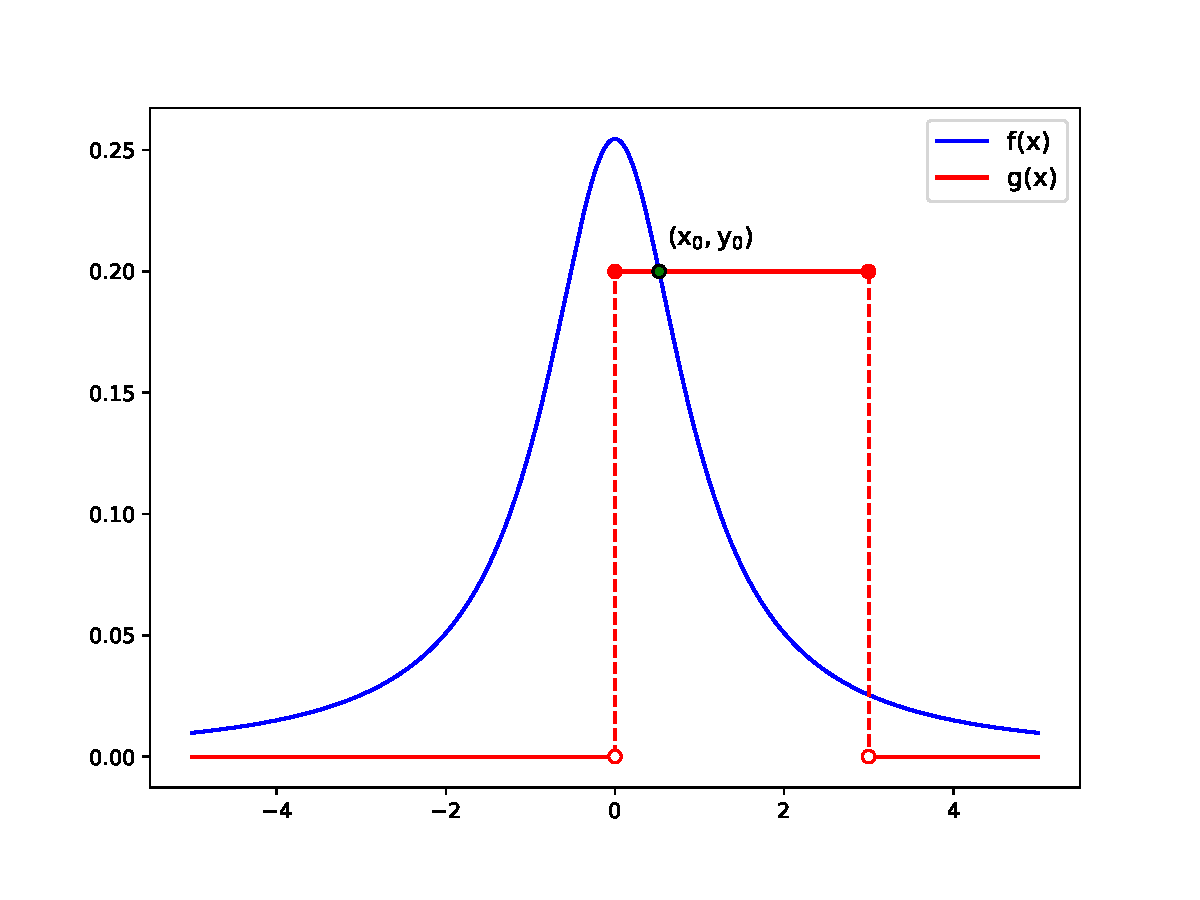
\includegraphics[width=\textwidth]{distribs.pdf}
        \caption{Графики распределений}
        \label{fig:distribs}
    \end{figure}

	Из рис. \ref{fig:distribs} видно, что
	\[
		g(x) \geq f(x) \iff x \in [x_0, 3].
	\]
	
	Таким образом, оптимальный классификатор будет иметь вид
	\[
		a^*(x) = 
		\left\{
		\begin{aligned}
			& -1, \ x \in (-\infty, x_0) \cup (3, +\infty) \\
			& +1, \ x \in [x_0, 3]
		\end{aligned}
		\right..
	\]
	
	Координату $x_0$ найдём следующим образом:
	\[
	\begin{gathered}
		f(x_0) = g(x_0) = 0.2 \implies \frac{0.8}{\pi (1 + {x_0}^2)} = 0.2 \implies \\
		\implies \pi (1 + {x_0}^2) = 4 \implies x_0 = \sqrt{\frac{4}{\pi} - 1}.
	\end{gathered}
	\]
	
    \section{Оптимальный средний риск}
    Имеем:
    \[
    	\begin{aligned}
    		R^* &= \iint L(a^*(x), y) p(x, y) \,dx\,dy \\
    		&= \iint \lambda_y [a^*(x) \neq y] p(x | y) P(y) \,dx\,dy \\
    		&= \iint \lambda_y (1 - [a^*(x) = y]) p(x | y) P(y) \,dx\,dy \\
    		&= \int \underset{y}{\min} \ \lambda_y p(x | y) P(y) \,dx\,dy \\
    		&= \int \underset{y}{\min} \left\{ \lambda_{-} p(x | y = -1) P(y = -1), \lambda_{+} p(x | y = +1) P(y = +1) \right\} \,dx\,dy \\
    		&= \int \underset{y}{\min} \left\{ f(x), g(x) \right\} \,dx\,dy.
    	\end{aligned}
    \]
    
    Аналогично пункту 1, получаем:
    \[
    	\begin{aligned}
    		R^* &= \int_{-\infty}^{x_0} g(x) \,dx + \int_{x_0}^{3} f(x) \,dx + \int_{3}^{+\infty} g(x) \,dx \\
    		&= \int_{0}^{x_0} 0.2 \,dx + \int_{x_0}^{3} \frac{0.8}{\pi (1 + x^2)} \,dx \\
    		&= 0.2 x_0 + \frac{0.8}{\pi} (\arctan{3} - \arctan{x_0}) \approx 0.299958 \approx 0.3.
    	\end{aligned}
    \]

    \section{Наивный байесовский классификатор}
    Имеем:
    \[
    	\begin{gathered}
    		a^*(x_1, x_2) = \underset{y}{\arg\!\max} \ P(y) p(x_1, x_2 | y), \\
    		p(x_1, x_2 | y) = p(x_1 | y) p(x_2 | y).
    	\end{gathered}
    \]
    
    По исходным данным нетрудно определить априорные вероятности классов:
    \[
    	\begin{gathered}
    		P(y = -1) = \frac{n_{-}}{n_{+} + n_{-}} = 0.4, \\
    		P(y = +1) = \frac{n_{+}}{n_{+} + n_{-}} = 0.6.
    	\end{gathered}
    \]
    
    Предположим, что исходные данные соответствуют нормальному распределению, то есть
    \[
    	\begin{gathered}
    		p(x_1 | y = -1) \sim N(\mu_{11}, \sigma_{11}^2), \ p(x_2 | y = -1) \sim N(\mu_{21}, \sigma_{21}^2), \\
    		p(x_1 | y = +1) \sim N(\mu_{12}, \sigma_{12}^2), \ p(x_2 | y = +1) \sim N(\mu_{22}, \sigma_{22}^2).
    	\end{gathered}
    \]
    
    Определим параметры распределений по следующим формулам:
    \[
    	\mu = \frac{1}{n} \sum_{i = 1}^{n} x_i, \ \sigma = \sqrt{\frac{1}{n - 1} \sum_{i = 1}^{n} (x_i - \mu)^2}.
    \]
    
    Получим следующие значения:
    \[
    	\begin{gathered}
    		\mu_{11} \approx -0.101, \ \sigma_{11} \approx 1.17, \\
    		\mu_{21} \approx 0.792, \ \sigma_{21} \approx 2.014, \\
    		\mu_{12} \approx 1.018, \ \sigma_{12} \approx 1.011, \\
    		\mu_{22} \approx 0.497, \ \sigma_{22} \approx 1.918.
    	\end{gathered}
    \]
    
    Имеем:
    \[
    	\begin{aligned}
    		a^*(x_1, x_2) &= \underset{y}{\arg\!\max} \ P(y) p(x_1, x_2 | y) \\
    		&= \underset{y}{\arg\!\max} \left\{ P(y = -1) p(x_1, x_2 | y = -1), P(y = +1) p(x_1, x_2 | y = +1) \right\} \\
    		&=\underset{y}{\arg\!\max} 
    		\left\{
    		\begin{aligned}
    			&P(y = -1) p(x_1 | y = -1) p(x_2 | y = -1), \\
    			&P(y = +1) p(x_1 | y = +1) p(x_2 | y = +1)
    		\end{aligned}
    		\right\} \\
    		&= \underset{y}{\arg\!\max} \left\{ f(x_1, x_2), g(x_1, x_2) \right\}.
    	\end{aligned}
    \]
    
    Очевидно, что
    \[
    	\begin{gathered}
    		f(x) = \frac{0.4}{2\pi \sigma_{11} \sigma_{21}} e^{-\frac{1}{2} \left[ (\frac{x_1 - \mu_{11}}{\sigma_{11}})^2 + (\frac{x_2 - \mu_{21}}{\sigma_{21}})^2 \right]}, \\
    		g(x) = \frac{0.6}{2\pi \sigma_{12} \sigma_{22}} e^{-\frac{1}{2} \left[ (\frac{x_1 - \mu_{12}}{\sigma_{12}})^2 + (\frac{x_2 - \mu_{22}}{\sigma_{22}})^2 \right]}.
    	\end{gathered}
    \]
    
    Таким образом, оптимальный наивный классификатор будет иметь вид
    \[
    	a^*(x_1, x_2) = 
    	\left\{
    	\begin{aligned}
    		& -1, \ f(x_1, x_2) \geq g(x_1, x_2) \\
    		& +1, \ f(x_1, x_2) < g(x_1, x_2)
    	\end{aligned}
    	\right..
    \]
    
\end{document}